\section{§15. Интеграл Коши}

Пусть $\gamma$ — кривая в $\mathbb{C}$. И функция $\varphi(\zeta)$ непрерывна на $\tilde{\gamma}$.

Тогда функция
\begin{equation} \label{eq:15.1}
    F(z) = \frac{1}{2\pi i} \int_{\gamma} \frac{\varphi(\zeta)}{\zeta - z} d\zeta
\end{equation}
называется \textit{интегралом Коши}.

Функция $F(z)$ определена для любого $z \in \mathbb{C} \setminus \tilde{\gamma}$.

\begin{figure}[h!]
    \centering
    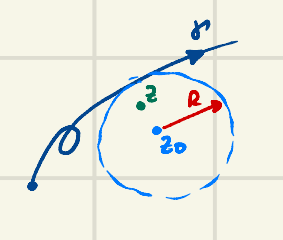
\includegraphics[width=0.3\textwidth]{images/placeholder_cauchy_curve.png}
    \caption{Кривая $\gamma$, точка $z$ внутри и $z_0$ с радиусом $R$.}
\end{figure}

\begin{theorem}{Теорема 1}
    Пусть $\tilde{\gamma} \cap B_R(z_0) = \varnothing$. Тогда в $B_R(z_0)$ функция \eqref{eq:15.1} представима степенным рядомом:
    \[
        F(z) = \sum_{n=0}^{\infty} c_n (z - z_0)^n,
    \]
    где
    \begin{equation} \label{eq:15.2}
        c_n = \frac{1}{2\pi i} \int_{\gamma} \frac{\varphi(\zeta)}{(\zeta - z_0)^{n+1}} d\zeta, \quad n=0, 1, 2, \dots
    \end{equation}
\end{theorem}

\begin{tproof}
    Зафиксируем $z \in B_R(z_0)$. Тогда для любого $\zeta \in \tilde{\gamma}$:
    \begin{equation} \label{eq:15.3}
        \frac{1}{\zeta - z} = \frac{1}{(\zeta - z_0) - (z - z_0)} = \frac{1}{\zeta - z_0} \cdot \frac{1}{1 - \frac{z - z_0}{\zeta - z_0}} = \sum_{n=0}^{\infty} \frac{(z - z_0)^n}{(\zeta - z_0)^{n+1}}
    \end{equation}
    
    Ряд \eqref{eq:15.3} сходится равномерно по $\zeta \in \tilde{\gamma}$, так как для любого $\zeta \in \tilde{\gamma}$:
    \[
        \left| \frac{(z - z_0)^n}{(\zeta - z_0)^{n+1}} \right| \le \frac{1}{R} \left( \frac{|z - z_0|}{R} \right)^n, \quad \text{a } \frac{|z - z_0|}{R} < 1
    \]
    и числовой ряд $\sum_{0}^{\infty} \frac{1}{R} \left( \frac{|z - z_0|}{R} \right)^n$ сходится (далее — признак Вейерштрасса).

    Домножим равенство \eqref{eq:15.3} на $\frac{\varphi(\zeta)}{2\pi i}$:
    \begin{equation} \label{eq:15.4}
        \frac{\varphi(\zeta)}{2\pi i (\zeta - z)} \equiv_{\tilde{\gamma}} \sum_{n=0}^{\infty} \frac{\varphi(\zeta) (z - z_0)^n}{2\pi i (\zeta - z_0)^{n+1}}
    \end{equation}
    
    Ряд \eqref{eq:15.4} также сходится равномерно на $\tilde{\gamma}$, так как $\frac{\varphi(\zeta)}{2\pi i}$ — ограниченная на $\tilde{\gamma}$ функция.
    
    Почленно интегрируем \eqref{eq:15.4}:
    \begin{equation} \label{eq:15.5}
        F(z) = \frac{1}{2\pi i} \int_{\gamma} \frac{\varphi(\zeta)}{\zeta - z} d\zeta = \sum_{n=0}^{\infty} \left( \frac{1}{2\pi i} \int_{\gamma} \frac{\varphi(\zeta)}{(\zeta - z_0)^{n+1}} d\zeta \right) (z - z_0)^n = \sum_{0}^{\infty} c_n (z - z_0)^n
    \end{equation}
    что и требовалось доказать.
\end{tproof}

\begin{conseq}
    Интеграл Коши $F(z) \in C^{\infty}(\mathbb{C} \setminus \tilde{\gamma})$.
\end{conseq}

\section{§16. Регулярные функции. Теорема Гурса}

\begin{definition}{Регулярная функция}
    Функция $f(z)$ называется:
    \begin{enumerate}
        \item \textit{регулярной на открытом множестве} $G \subset \mathbb{C}$, если $f$ дифференцируема в $G$.
        \item \textit{регулярной на множестве} $E$, если существует открытое множество $G \supset E$, на котором $f$ регулярна.
        \item В частности, $f$ регулярна в точке $z_0$, если $f$ регулярна на одноточечном множестве $\{z_0\}$.
    \end{enumerate}
\end{definition}

\begin{note}{}
    Пункт 3) можно равносильно сформулировать так: $f(z)$ регулярна в т. $z_0$, если $f$ дифференцируема в некоторой $B_{\varepsilon}(z_0)$.
\end{note}

\begin{note}{}
    Дифференцируемость $f$ в точке $z_0$ необходима, но не достаточна для регулярности $f$ в $z_0$.
\end{note}

\textbf{Пример:} $f = |z|^2$. Дифференцируема в единственной точке $z=0$ и не регулярна ни в одной точке.

\begin{theorem}{Теорема Гурса}
    Пусть $f(z)$ регулярна в замкнутом прямоугольнике $\Pi = \{z : a \le \text{Re} z \le b, ~ c \le \text{Im} z \le d\}$.
    Тогда:
    \begin{equation} \label{eq:16.1}
        \oint_{\partial \Pi} f(z) dz = 0
    \end{equation}
    (имеется в виду интеграл по $\gamma = \partial \Pi$ обход против часовой стрелки).
\end{theorem}

\begin{figure}[h!]
    \centering
    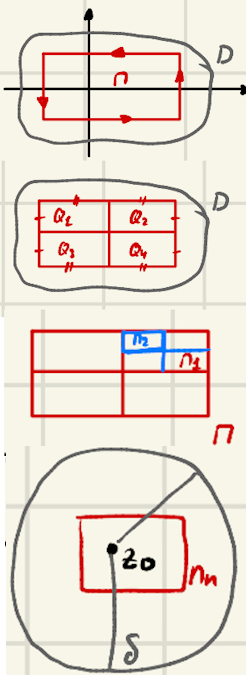
\includegraphics[width=0.4\textwidth]{images/placeholder_goursat_rect.png}
    \caption{Контур $\partial \Pi$ и разбиение прямоугольника.}
\end{figure}

\begin{tproof}
    Пусть $|\int_{\partial \Pi} f dz| = M$.
    
    Разбиваем $\Pi$ на 4 равных прямоугольника $Q_1, Q_2, Q_3, Q_4$.
    \[
        \int_{\partial \Pi} f dz = \sum_{k=1}^{4} \int_{\partial Q_k} f dz \implies M = \left| \int_{\partial \Pi} f dz \right| \le \sum_{k=1}^{4} \left| \int_{\partial Q_k} f dz \right|
    \]
    Следовательно, $\exists Q_k$: $|\int_{\partial Q_k} f dz| \ge \frac{M}{4}$. Обозначим этот $Q_k$ через $\Pi_1$.
    
    Аналогично, делим $\Pi_1$ на 4 части, находим $\Pi_2$:
    \[
        \exists \Pi_2 : \left| \int_{\partial \Pi_2} f dz \right| \ge \frac{M}{4^2}
    \]
    Получаем последовательность вложенных прямоугольников:
    \[
        \Pi \supset \Pi_1 \supset \Pi_2 \supset \dots \supset \Pi_n \supset \Pi_{n+1} \supset \dots
    \]
    для которых выполнено:
    \[
        \left| \int_{\partial \Pi_n} f dz \right| \ge \frac{M}{4^n}.
    \]
    
    Если $L$ — периметр прямоугольника $\Pi$, то $\frac{L}{2^n}$ — периметр прямоугольника $\Pi_n$.
    
    По теореме (из мат. анализа) о вложенных отрезках: $\exists z_0 \in \bigcap_{n=1}^{\infty} \Pi_n \in \Pi$.
    
    Т.к. $f(z)$ дифференцируема в т. $z_0$, то в некоторой $B_{\delta_0}(z_0)$ верно представление:
    \begin{equation} \label{eq:16.3}
        f(z) = f(z_0) + f'(z_0)(z - z_0) + |z - z_0| \cdot \alpha(z)
    \end{equation}
    где $\alpha(z)$ непрерывна в $B_{\delta_0}(z_0)$ и $\alpha(z_0) = 0$.

    Зададим конкретное $\varepsilon > 0$. Под него подберем $\delta > 0$: при $z \in B_{\delta}(z_0)$ ($ \delta \in (0, \delta_0)$): $|\alpha(z)| < \varepsilon$.
    Под это $\delta$ подберем $n$: $\frac{L}{2^n} < \delta$.
    
    \textbf{Утверждение:} $\forall z \in \Pi_n$ верно: $z \in B_{\delta}(z_0)$.
    \textbf{Обоснование:} Для любого $z \in \Pi_n$:
    \[
        |z - z_0| < \text{диагональ} < \text{периметр} = \frac{L}{2^n} < \delta.
    \]
    
    Рассмотрим интеграл по $\partial \Pi_n$:
    \[
        \int_{\partial \Pi_n} f(z) dz \overset{\eqref{eq:16.3}}{=} \int_{\partial \Pi_n} \left[ f(z_0) + f'(z_0)(z - z_0) \right] dz + \int_{\partial \Pi_n} |z - z_0| \cdot \alpha(z) dz
    \]
    Первый интеграл равен $0$, т.к. подынтегральная функция $[\dots]$ непрерывна и имеет первообразную $f(z_0) \cdot z + f'(z_0) \cdot \frac{(z - z_0)^2}{2}$.
    
    Тогда оцениваем оставшуюся часть:
    \[
        \left| \int_{\partial \Pi_n} f(z) dz \right| = \left| \int_{\partial \Pi_n} |z - z_0| \cdot \alpha(z) dz \right| \le \max_{z \in \partial \Pi_n} (|z - z_0| \cdot |\alpha(z)|) \cdot \text{длина}(\partial \Pi_n) \le
    \]
    \[
        \le \frac{L}{2^n} \cdot \varepsilon \cdot \frac{L}{2^n} = \frac{\varepsilon L^2}{4^n}.
    \]
    
    Таким образом:
    \[
        \frac{M}{4^n} \le \left| \int_{\partial \Pi_n} f dz \right| \le \frac{\varepsilon L^2}{4^n} \implies 0 \le M \le \varepsilon L^2.
    \]
    
    В силу произвольности $\varepsilon > 0$: $M = 0 \implies \int_{\partial \Pi} f dz = 0$, ч.т.д.
\end{tproof}

\section{§17. Правила замены комплексной переменной под знаком интеграла}

Пусть функция $w = F(z)$ преобразует кривую $\gamma$ в кривую $\Gamma$.
Тогда при некоторых условиях верно:
\begin{equation} \label{eq:17.1}
    \int_{\Gamma} \Phi(w) dw = \int_{\gamma} \Phi(F(z)) F'(z) dz
\end{equation}

Выясним эти условия.

\begin{statement}{Утверждение 1}
    Пусть $\gamma: z = z(t), ~ \alpha \le t \le \beta$ — КНГ-кривая (кусочно-непрерывно гладкая).
    Функция $w = F(z)$ непрерывно дифференцируема в области $G$ и $\tilde{\gamma} \subset G$.
    
    Тогда $\Gamma$:
    \begin{equation} \label{eq:17.2}
        w(t) = F(z(t)), \quad \alpha \le t \le \beta
    \end{equation}
    — тоже КНГ-кривая.
\end{statement}

\begin{proof}
    а) Функция $w(t) \in C[\alpha, \beta]$.
    б) $w'(t) = \underbrace{F'(z(t))}_{\text{непрер.}} \cdot \underbrace{z'(t)}_{\text{кус-непрер.}} $ — кусочно-непрерывна.
\end{proof}

\begin{statement}{Утверждение 2}
    Пусть выполнены условия Утв. 1 и $\Phi(w)$ такова, что $\Phi(w(t)) \in C[\alpha, \beta]$.
    Тогда верна формула \eqref{eq:17.1}.
\end{statement}

\begin{proof}
    \[
        \{\text{л.ч. ф-лы } \eqref{eq:17.1} \} \triangleq \int_{\alpha}^{\beta} \Phi(w(t)) w'(t) dt \overset{\text{\circled{3}}}{=} \int_{\alpha}^{\beta} \Phi(F(z(t))) F'(z(t)) \cdot z'(t) dt \triangleq \{ \text{пр. часть ф-лы } \eqref{eq:17.1} \}
    \]
\end{proof}

\textbf{Пример:}
Пусть $\gamma_1: z = t - i, ~ -1 \le t \le 1, ~ z'(t) = 1$.
\[
    \int_{\gamma_1} \frac{dz}{z} = \int_{-1}^{1} \frac{1 \cdot dt}{t - i} = \int_{-1}^{1} \frac{t + i}{t^2 + 1} dt = \underbrace{\int_{-1}^{1} \frac{t dt}{t^2 + 1}}_{=0} + i \int_{-1}^{1} \frac{dt}{t^2 + 1} = i \frac{\pi}{2}.
\]
Аналогично (упр.): $\int_{\gamma_k} \frac{dz}{z} = i \frac{\pi}{2}$.
Следовательно, для $\gamma = \gamma_1 \gamma_2 \gamma_3 \gamma_4$: $\oint_{\gamma} \frac{dz}{z} = 2\pi i$.

\begin{center}
    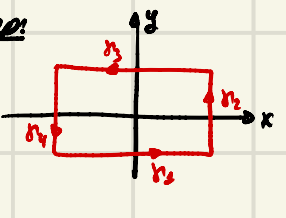
\includegraphics[width=0.4\textwidth]{images/placeholder_square_contour.png}
    \captionof{figure}{Квадратный контур вокруг начала координат.}
\end{center}

Применим Утв. 1, 2 для случая $\gamma$ — контур из Примера 1.
$F(z) = a + z \cdot \delta$, где $a \in \mathbb{C}, \delta > 0$.
$\Phi(w) = \frac{1}{w - a}$ (проверив все усл. Утв 1, 2 выполн.)

Тогда $F(z)$ преобразует кривую $\gamma$ в кривую $\Gamma$: (квадрат со стороной $2\delta$ с центром в $a$).

\begin{center}
    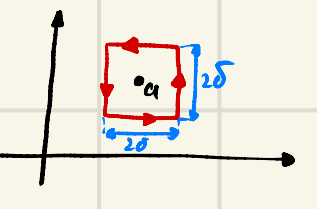
\includegraphics[width=0.4\textwidth]{images/placeholder_square_2_delta.png}
    \captionof{figure}{Квадрат со стороной $2\delta$ с центром в $a$.}
\end{center}

\[
    \int_{\Gamma} \frac{dw}{w - a} = \int_{\gamma} \frac{\delta \cdot dz}{(a + z\delta) - a} = \int_{\gamma} \frac{dz}{z} = 2\pi i.
\]

\section{§18. Интегральная формула Коши для прямоугольной области. Бесконечная дифференцируемость регулярных функций}

\begin{theorem}{Теорема 1}
    Пусть $D = \{ z = x + iy \mid a \le x \le b, ~ c \le y \le d \}$.
    $f(z)$ регулярна в $\bar{D}$. Тогда для любого $z_0 \in D$:
    \begin{equation} \label{eq:18.1}
        f(z_0) = \frac{1}{2\pi i} \oint_{\partial D} \frac{f(z)}{z - z_0} dz, \quad \text{обход } \partial D \text{ против часов.}
    \end{equation}
\end{theorem}

(Пригодится: $\forall \delta > 0$ \quad $\int_{\partial Q_{\delta}(z_0)} \frac{dz}{z - z_0} = 2\pi i$, где $Q_{\delta}(z_0) = \{ z \mid |\text{Re} z - \text{Re} z_0| \le \delta, ~ |\text{Im} z - \text{Im} z_0| \le \delta \}$)

\begin{tproof}
    Зафиксируем $\varepsilon > 0$. Под это $\varepsilon$ подберем $\delta > 0$, так что $\forall z \in Q_{\delta}(z_0): |f(z) - f(z_0)| \le \varepsilon$ (это нужно, т.к. $f$ непрер.).
    
    \begin{center}
        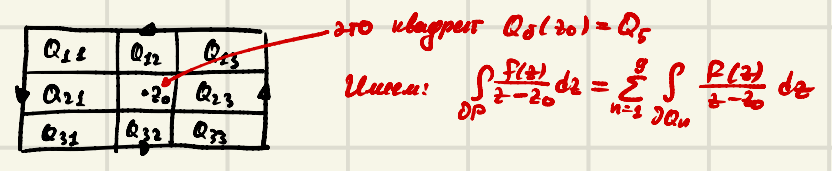
\includegraphics[width=0.4\textwidth]{images/placeholder_domain_subdivision.png}
        \captionof{figure}{Разбиение области $D$, выделен квадрат $Q_{\delta}(z_0) = Q_s$.}
    \end{center}

    Имеем: $\int_{\partial D} \frac{f(z)}{z - z_0} dz = \sum_{k=1}^{S} \int_{\partial Q_k} \frac{f(z)}{z - z_0} dz$.
    
    При $k \ne s$: $\int_{\partial Q_k} \frac{f(z)}{z - z_0} dz = 0$ по Тл Гурса, т.к. ф-я $g(z) = \frac{f(z)}{z - z_0}$ рег. в $\bar{Q}_k, k \ne s$.
    
    Итак верно:
    \begin{equation} \label{eq:18.2}
        \int_{\partial D} \frac{f(z)}{z - z_0} dz = \int_{\partial Q_s(z_0)} \frac{f(z)}{z - z_0} dz
    \end{equation}
    
    Имеем
    \[
        \left| 2\pi i f(z_0) - \int_{\partial D} \frac{f(z)}{z - z_0} dz \right| = \left| 2\pi i \cdot f(z_0) - \int_{\partial Q_{\delta}(z_0)} \frac{f(z)}{z - z_0} dz \right| \overset{(\ref{eq:18.1}a)}{=}
    \]
    \[
        = \left| f(z_0) \int_{\partial Q_{\delta}(z_0)} \frac{dz}{z - z_0} - \int_{\partial Q_{\delta}(z_0)} \frac{f(z) dz}{z - z_0} \right| = \left| \int_{\partial Q_{\delta}(z_0)} \frac{f(z_0) - f(z)}{z - z_0} dz \right| \le
    \]
    \[
        \le \max_{z \in Q_{\delta}(z_0)} \left| \frac{f(z) - f(z_0)}{z - z_0} \right| \cdot 8\delta \le \frac{\varepsilon}{\delta} \cdot 8\delta = 8\varepsilon.
    \]
    
    $\implies |\dots| = 0 \implies$ ф-ла \eqref{eq:18.1} ч.т.д.
\end{tproof}

\section{§19. Интегральная теорема Коши}

\begin{theorem}{Теорема 1}
    Пусть $f(z)$ регулярна в односвязной области $G$, $\gamma$ — кусочно-гладкая замкнутая кривая, $\tilde{\gamma} \subset G$.
    
    Тогда:
    \begin{equation} \label{eq:19.1}
        \oint_{\gamma} f(z) dz = 0
    \end{equation}
\end{theorem}

\begin{tproof}
    Пусть $f(z) = u(x,y) + i v(x,y)$.
    
    В силу Теоремы 2 из §18, регулярная функция $f(z)$ имеет производные всех порядков в $G$. Следовательно, в частности, $u(x,y), v(x,y) \in C^1(G)$.
    
    Имеем интеграл:
    \[
        \oint_{\gamma} f(z) dz = \oint_{\gamma} (u + iv)(dx + i dy) = \underbrace{\oint_{\gamma} (u dx - v dy)}_{I_1} + i \underbrace{\oint_{\gamma} (v dx + u dy)}_{I_2}
    \]
    
    В силу теоремы из матанализа (формула Грина):
    \[
        \oint P dx + Q dy = \iint_{D} \left( \frac{\partial Q}{\partial x} - \frac{\partial P}{\partial y} \right) dx dy,
    \]
    где $D$ — область, ограниченная контуром $\gamma$ (так как $G$ односвязна, $D \subset G$).
    
    Если $\tilde{\gamma}$ лежит в односвязной области, в которой $P(x,y), Q(x,y) \in C^1(G)$ и $\frac{\partial Q}{\partial x} \equiv \frac{\partial P}{\partial y}$.
    
    Применим для $I_1$, положив $P = u, ~ Q = -v$.
    В силу условий Коши-Римана $u_y = -v_x \implies -v_x = u_y$.
    \[
        I_1 = \iint_{D} \left( -\frac{\partial v}{\partial x} - \frac{\partial u}{\partial y} \right) dx dy = \iint_{D} (u_y - u_y) dx dy = 0.
    \]
    
    Аналогично доказывается, что $I_2 = 0$ из второго условия Коши-Римана ($u_x = v_y$).
    
    Следовательно, $\oint_{\gamma} f(z) dz = 0$, ч.т.д.
\end{tproof}

\textbf{Примеры областей:}
\begin{enumerate}
    \item $G_1 = \{z : |z| > 1\} \cup \{\infty\}$ — неограниченная односвязная область (но теорема требует конечности контура или аккуратного определения).
    \item $G_2 = \{z : 1 < |z| < 2\}$ — ограниченная многосвязная область.
    \item $G_3 = B_{\delta}^{\circ}(0)$ (проколотая окрестность) — не односвязная.
    \item $G_4$ — верхняя полуплоскость — односвязная область.
\end{enumerate}

\textbf{Пример:} $G = \{z \mid \frac{1}{2} < |z| < 2 \}$, $f(z) = \frac{1}{z}$.
$\gamma : |z| = 1$, обход против часовой стрелки.
Тогда $\tilde{\gamma} \subset G$, однако $\oint_{|z|=1} \frac{dz}{z} = 2\pi i \ne 0$.
$\implies$ условие односвязности существенно.

\begin{conseq}
    Если $f(z)$ регулярна в односвязной области $G \subset \mathbb{C}$, то $f$ имеет первообразную в $G$.
\end{conseq}
\begin{proof}
    1) $f$ — регулярна $\implies f$ непрерывна.
    2) $f$ — непрерывна и $\oint_{\gamma} f dz = 0 ~ \forall$ контура $\tilde{\gamma} \subset G \implies f$ имеет первообразную. Ч.т.д.
\end{proof}

\subsection*{Определения (геометрические)}

\begin{definition}{Гладкая и кусочно-гладкая кривая}
    Непрерывно дифференцируемая кривая называется \textit{гладкой}, если $z'(t) \ne 0, ~ \alpha \le t \le \beta$ (т.е. существует касательная в каждой точке).
    
    $\gamma$ — \textit{кусочно-гладкая}, если составлена из конечного числа гладких кривых.
\end{definition}

\begin{definition}{Область с простой границей (ОСПГ)}
    Область $G \subset \mathbb{C}$ называется \textit{областью с простой границей} (ОСПГ), если $\partial G = \tilde{\gamma}_1 \cup \dots \cup \tilde{\gamma}_n$, где $\tilde{\gamma}_k$ — носители простых кусочно-гладких контуров, причем $\tilde{\gamma}_k \cap \tilde{\gamma}_l = \varnothing, ~ k \ne l$.
\end{definition}

\begin{definition}{Ориентация границы}
    $\partial G$ ($G$ — область) — положительно ориентирована, если при обходе любой граничной кривой область остается слева.
\end{definition}

\begin{theorem}{Теорема 2 (Интегральная теорема Коши для ограниченной ОСПГ)}
    Пусть:
    \begin{enumerate}
        \item $G \Subset \mathbb{C}$ — ограниченная ОСПГ с границей, ориентированной положительно.
        \item $f(z)$ регулярна в $\bar{G}$ (т.е. в $G$ и некоторой окрестности границы).
    \end{enumerate}
    Тогда:
    \begin{equation} \label{eq:19.3}
        \oint_{\partial G} f(z) dz = 0 \quad \left( \oint_{\partial G} f dz \triangleq \sum_{k=1}^{n} \oint_{\gamma_k} f dz \right)
    \end{equation}
\end{theorem}

\begin{center}
    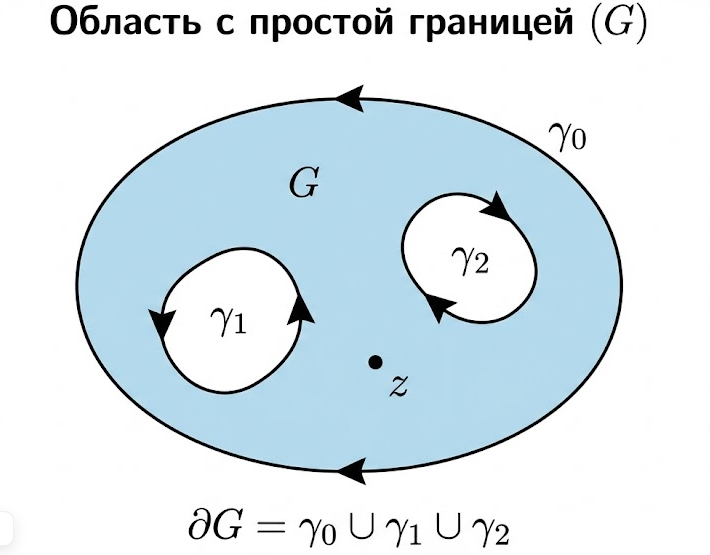
\includegraphics[width=0.4\textwidth]{images/placeholder_ospg.png}
    \captionof{figure}{Область с простой границей (ОСПГ).}
\end{center}

\begin{tproof}
    Из условия следует: $f(z)$ имеет производные всех порядков в некотором открытом $D \supset \bar{G}$.
    Пусть $f(z) = u(x,y) + i v(x,y)$. Тогда $u(x,y), v(x,y)$ имеют, в частности, производные первого порядка в $D$.
    
    По свойству интеграла:
    \[
        \oint_{\partial G} f dz = \oint_{\partial G} (u dx - v dy) + i \oint_{\partial G} (v dx + u dy).
    \]
    Применяем формулу Грина для многосвязной области (она справедлива для таких областей).
    Обозначим $I_1 = \oint_{\partial G} (u dx - v dy)$. Здесь $P=u, Q=-v$.
    \[
        I_1 = \iint_{G} \left( -\frac{\partial v}{\partial x} - \frac{\partial u}{\partial y} \right) dx dy.
    \]
    Так как $f$ регулярна, выполнены условия Коши-Римана $u_y = -v_x$.
    \[
        I_1 = \iint_{G} (u_y - u_y) dx dy = 0.
    \]
    Аналогично доказывается $I_2 = 0$. Ч.т.д.
\end{tproof}

\begin{note}{}
    Ни одна из Теорем (И.Т.К.) №1 и №2 не является более общей по отношению к другой. Теорема 1 требует односвязности, но допускает более плохие границы (в пределе). Теорема 2 допускает многосвязность, но требует регулярности вплоть до границы (в замыкании).
\end{note}


\section{§20. Интегральная формула Коши для ограниченной ОСПГ. Формулы для производных. Разложение в степенной ряд}

\begin{theorem}{Теорема 1}
    Пусть:
    \begin{enumerate}
        \item $G$ — ограниченная ОСПГ.
        \item $f(z)$ регулярна в $\bar{G}$.
        \item $a \in G$.
        \item $\partial G$ ориентирована положительно.
    \end{enumerate}
    Тогда:
    \begin{equation} \label{eq:20.1}
        f(a) = \frac{1}{2\pi i} \oint_{\partial G} \frac{f(z)}{z - a} dz
    \end{equation}
\end{theorem}

\begin{tproof}
    Выберите прямоугольник $\Pi$ такой, что $a \in \Pi, ~ \bar{\Pi} \subset G$.
    Пусть $\gamma$ — граничная кривая прямоугольника $\Pi$, ориентированная положительно относительно $\Pi$.
    
    Рассмотрим область $G \setminus \bar{\Pi}$. Это ОСПГ, её граничные кривые (ориентированные положительно относительно области $G \setminus \bar{\Pi}$) таковы: $\gamma_1, \dots, \gamma_n$ (внешняя граница $\partial G$) и $\gamma^{-1}$ (граница прямоугольника, проходимая по часовой стрелке).
    
    \begin{center}
        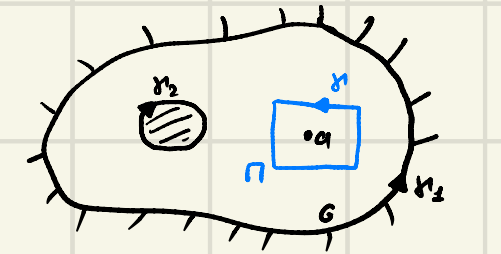
\includegraphics[width=0.4\textwidth]{images/placeholder_punctured_domain.png}
        \captionof{figure}{Область $G$ с вырезанным прямоугольником $\Pi$ вокруг точки $a$.}
    \end{center}

    Функция $\frac{f(z)}{z - a}$ регулярна в замыкании области $G \setminus \bar{\Pi}$ (так как особая точка $a$ выброшена).
    Применим к ней Теорему 2 из §19:
    \begin{equation} \label{eq:20.2}
        \sum_{k=1}^{n} \oint_{\gamma_k} \frac{f(z)}{z - a} dz + \oint_{\gamma^{-1}} \frac{f(z)}{z - a} dz = 0
    \end{equation}
    
    Первое слагаемое — это интеграл по $\partial G$. Второе слагаемое перенесем вправо (меняя знак, т.е. меняя ориентацию на $\gamma$):
    \[
        \oint_{\partial G} \frac{f(z)}{z - a} dz = \oint_{\gamma} \frac{f(z)}{z - a} dz.
    \]
    
    По интегральной формуле Коши для прямоугольной области (см. §18), правая часть равна:
    \[
        \oint_{\gamma} \frac{f(z)}{z - a} dz = 2\pi i f(a).
    \]
    
    Следовательно:
    \[
        \oint_{\partial G} \frac{f(z)}{z - a} dz = 2\pi i f(a) \implies f(a) = \frac{1}{2\pi i} \oint_{\partial G} \frac{f(z)}{z - a} dz, \quad \text{ч.т.д.}
    \]
\end{tproof}

Итак, доказано:
\[
    f(z) = \frac{1}{2\pi i} \oint_{\partial G} \frac{f(\zeta)}{\zeta - z} d\zeta
\]
при условиях: $G$ — огр. ОСПГ, $f(\zeta)$ рег. в $\bar{G}$, $z \in G$.

Интеграл Коши (§15): $F(z) = \frac{1}{2\pi i} \int_{\gamma} \frac{\varphi(\zeta)}{\zeta - z} d\zeta$ — эта функция бесконечно дифференцируема в т. $z \in \mathbb{C} \setminus \tilde{\gamma}$.
Так как правая часть формулы (1) есть интеграл Коши, то в силу Теоремы из §15, $f(z) \in C^{\infty}(G)$.

\begin{theorem}{Теорема 2}
    Пусть $f(z)$ регулярна в области $G$.
    Тогда $f(z) \in C^{\infty}(G)$.
\end{theorem}
\begin{tproof}
    Зафиксируем т. $z_0 \in G$ и возьмем прямоугольную область $D$: $z_0 \in D, ~ \bar{D} \subset G$.
    
    В силу формулы (1) (так как правая часть есть интеграл Коши), функция $f(z)$ имеет производные всех порядков для $z \in D$, в частности в т. $z_0$.
    В силу произвольности $z_0$ теорема доказана.
\end{tproof}

\begin{conseq}
    Для интеграла Коши (см. §15) доказано:
    \[
        F^{(n)}(z) = \frac{n!}{2\pi i} \int_{\gamma} \frac{\varphi(\zeta)}{(\zeta - z)^{n+1}} d\zeta, \quad z \notin \tilde{\gamma}.
    \]
    Поэтому в силу (1) имеем $\forall n$:
    \begin{equation} \label{eq:20.3}
        f^{(n)}(z) = \frac{n!}{2\pi i} \oint_{\partial G} \frac{f(\zeta)}{(\zeta - z)^{n+1}} d\zeta \quad \text{для } z \in G,
    \end{equation}
    если $f$ регулярна в $\bar{G}$ (замыкании прямоугольной области $G$).
    Эта формула называется \textit{формулой Коши для производных}.
\end{conseq}

\begin{conseq}
    В условиях Т.1 верно:
    \[
        f^{(n)}(a) = \frac{n!}{2\pi i} \oint_{\partial G} \frac{f(z)}{(z - a)^{n+1}} dz, \quad \forall n \in \mathbb{N}.
    \]
\end{conseq}
\begin{proof}
    Обозначим $F_k(a) = \frac{1}{2\pi i} \int_{\gamma_k} \frac{f(z)}{z - a} dz$. Из §15 следует: $\forall a \notin \tilde{\gamma}_k$:
    \[
        F_k^{(n)}(a) = \frac{n!}{2\pi i} \int_{\gamma_k} \frac{f(z)}{(z - a)^{n+1}} dz.
    \]
    В силу $f(a) = \sum_{k=1}^{n} F_k(a)$, складывая равенства при $k=1..n$, получаем требуемое.
\end{proof}

\begin{theorem}{Теорема 3 (О разложении регулярной функции в степенной ряд)}
    Пусть $f(z)$ регулярна в круге $B_R(z_0), ~ R > 0$.
    Тогда существует единственное разложение функции $f(z)$ в степенной ряд
    \begin{equation} \label{eq:20.4}
        f(z) = \sum_{n=0}^{\infty} c_n (z - z_0)^n
    \end{equation}
    в этом круге.
\end{theorem}

\begin{tproof}
    Зафиксируем любое $0 < R_1 < R$. Тогда $f(z)$ регулярна в $B_{R_1}(z_0)$.
    Но $B_{R_1}(z_0)$ — ОСПГ, по интегральной формуле Коши для ОСПГ:
    \begin{equation} \label{eq:20.5}
        f(z) = \frac{1}{2\pi i} \oint_{\partial B_{R_1}(z_0)} \frac{f(\zeta)}{\zeta - z} d\zeta
    \end{equation}
    
    Правая часть формулы \eqref{eq:20.5} есть интеграл Коши, в котором $\gamma = \partial B_{R_1}(z_0)$.
    Так как $B_{R_1}(z_0) \cap \partial B_{R_1}(z_0) = \varnothing$, то из §15 следует, что этот интеграл Коши может быть представлен суммой:
    \[
        \sum_{n=0}^{\infty} c_n (z - z_0)^n.
    \]
    
    Итак, $f(z) = \sum_{n=0}^{\infty} c_n (z - z_0)^n$ в $B_{R_1}(z_0)$, где $c_n = \frac{f^{(n)}(z_0)}{n!}$ (единственность следует из формулы Тейлора для коэффициентов).
    
    Т.к. $R_1$ произвольно $\implies$ разложение справедливо во всём круге.
\end{tproof}